\documentclass{standalone}
\usepackage{tikz}
\usetikzlibrary{patterns, positioning}


\begin{document}
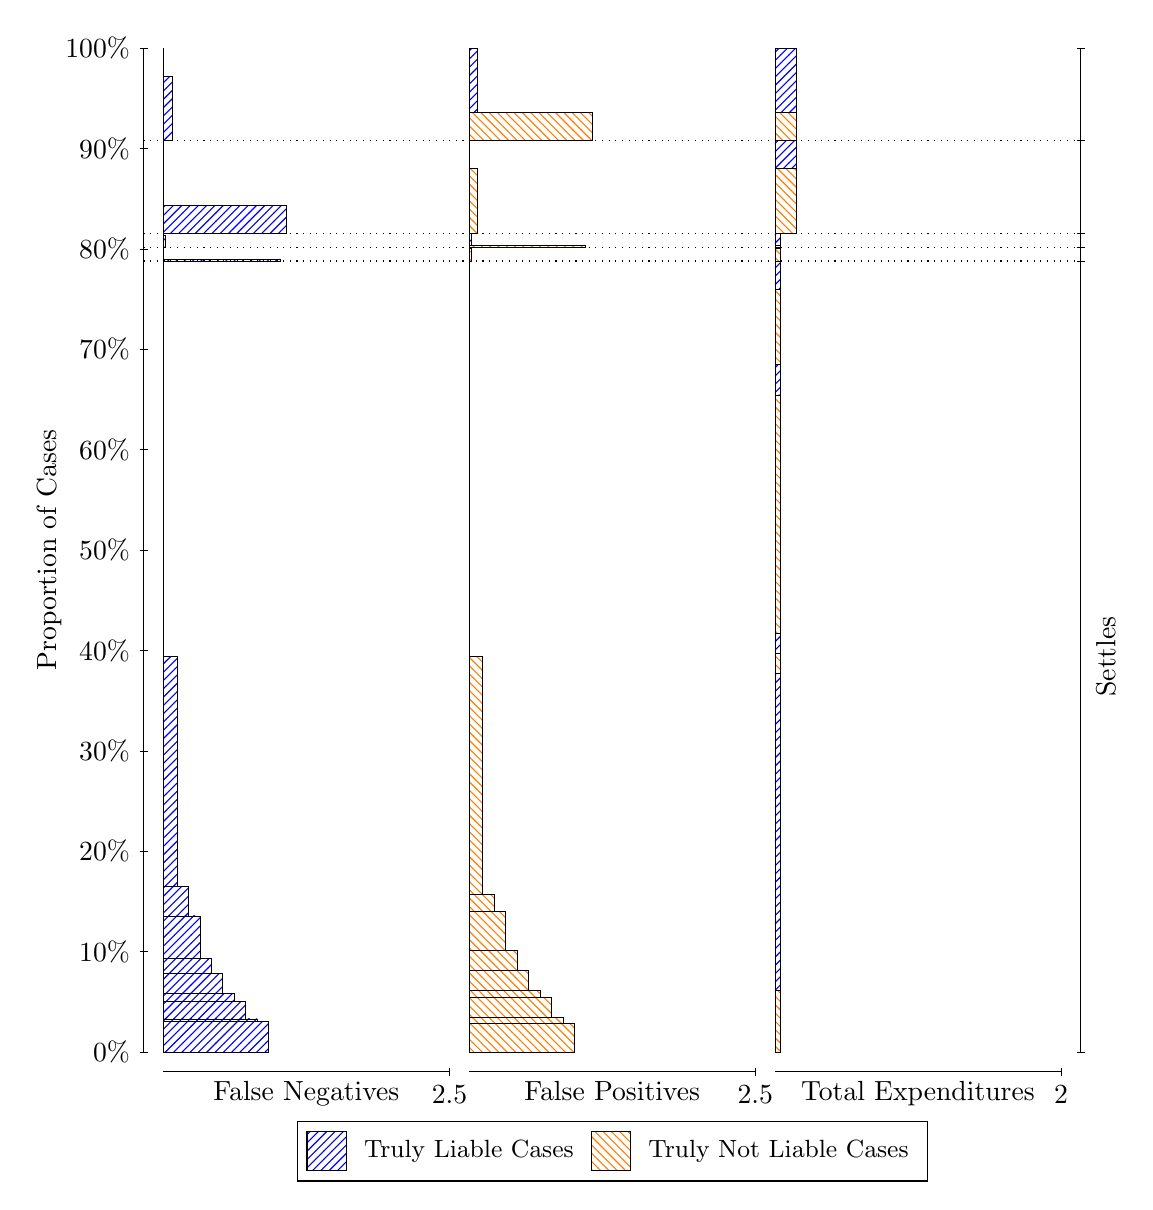
\begin{tikzpicture}
\draw[black, very thin] (1.5,1.75) -- (1.5,14.5);
\node[rotate=90, text=black, anchor=center] at (0.3, 8.125) {Proportion of Cases};
\draw[black, very thin] (1.45,1.75) -- (1.55,1.75);
\node[text=black, anchor=east] at (1.45, 1.75) {0\%};
\draw[black, very thin] (1.45,3.025) -- (1.55,3.025);
\node[text=black, anchor=east] at (1.45, 3.025) {10\%};
\draw[black, very thin] (1.45,4.3) -- (1.55,4.3);
\node[text=black, anchor=east] at (1.45, 4.3) {20\%};
\draw[black, very thin] (1.45,5.575) -- (1.55,5.575);
\node[text=black, anchor=east] at (1.45, 5.575) {30\%};
\draw[black, very thin] (1.45,6.85) -- (1.55,6.85);
\node[text=black, anchor=east] at (1.45, 6.85) {40\%};
\draw[black, very thin] (1.45,8.125) -- (1.55,8.125);
\node[text=black, anchor=east] at (1.45, 8.125) {50\%};
\draw[black, very thin] (1.45,9.4) -- (1.55,9.4);
\node[text=black, anchor=east] at (1.45, 9.4) {60\%};
\draw[black, very thin] (1.45,10.675) -- (1.55,10.675);
\node[text=black, anchor=east] at (1.45, 10.675) {70\%};
\draw[black, very thin] (1.45,11.95) -- (1.55,11.95);
\node[text=black, anchor=east] at (1.45, 11.95) {80\%};
\draw[black, very thin] (1.45,13.225) -- (1.55,13.225);
\node[text=black, anchor=east] at (1.45, 13.225) {90\%};
\draw[black, very thin] (1.45,14.5) -- (1.55,14.5);
\node[text=black, anchor=east] at (1.45, 14.5) {100\%};

\draw[black, very thin] (13.4,1.75) -- (13.4,14.5);
\draw[black, very thin] (13.35,1.75) -- (13.45,1.75);
\node[anchor=west] at (13.35, 1.75) {};
\draw[black, very thin] (13.35,11.795) -- (13.45,11.795);
\node[anchor=west] at (13.35, 11.795) {};
\draw[black, very thin] (13.35,11.971) -- (13.45,11.971);
\node[anchor=west] at (13.35, 11.971) {};
\draw[black, very thin] (13.35,12.146) -- (13.45,12.146);
\node[anchor=west] at (13.35, 12.146) {};
\draw[black, very thin] (13.35,13.326) -- (13.45,13.326);
\node[anchor=west] at (13.35, 13.326) {};
\draw[black, very thin] (13.35,14.5) -- (13.45,14.5);
\node[anchor=west] at (13.35, 14.5) {};

\draw[black, very thin, pattern color=blue, pattern=north east lines] (1.75,1.75) rectangle (3.0852,2.1368);
\draw[black, very thin, pattern color=blue, pattern=north east lines] (1.75,2.1368) rectangle (2.9399,2.1713);
\draw[black, very thin, pattern color=blue, pattern=north east lines] (1.75,2.1713) rectangle (2.7946,2.3896);
\draw[black, very thin, pattern color=blue, pattern=north east lines] (1.75,2.3896) rectangle (2.6492,2.4934);
\draw[black, very thin, pattern color=blue, pattern=north east lines] (1.75,2.4934) rectangle (2.5039,2.7482);
\draw[black, very thin, pattern color=blue, pattern=north east lines] (1.75,2.7482) rectangle (2.3586,2.9386);
\draw[black, very thin, pattern color=blue, pattern=north east lines] (1.75,2.9386) rectangle (2.2133,3.4785);
\draw[black, very thin, pattern color=blue, pattern=north east lines] (1.75,3.4785) rectangle (2.0679,3.8487);
\draw[black, very thin, pattern color=blue, pattern=north east lines] (1.75,3.8487) rectangle (1.9226,6.7756);
\draw[black, very thin, pattern color=orange, pattern=north west lines] (1.75,6.7756) rectangle (1.75,11.795);
\draw[black, very thin, pattern color=blue, pattern=north east lines] (1.75,11.795) rectangle (3.2306,11.815);
\draw[black, very thin, pattern color=orange, pattern=north west lines] (1.75,11.815) rectangle (1.75,11.971);
\draw[black, very thin, pattern color=blue, pattern=north east lines] (1.75,11.971) rectangle (1.7773,12.127);
\draw[black, very thin, pattern color=orange, pattern=north west lines] (1.75,12.127) rectangle (1.75,12.146);
\draw[black, very thin, pattern color=blue, pattern=north east lines] (1.75,12.146) rectangle (3.3123,12.505);
\draw[black, very thin, pattern color=orange, pattern=north west lines] (1.75,12.505) rectangle (1.75,13.326);
\draw[black, very thin, pattern color=blue, pattern=north east lines] (1.75,13.326) rectangle (1.859,14.141);
\draw[black, very thin, pattern color=orange, pattern=north west lines] (1.75,14.141) rectangle (1.75,14.5);
\draw[black, very thin, pattern color=orange, pattern=north west lines] (5.6333,1.75) rectangle (6.9686,2.1179);
\draw[black, very thin, pattern color=orange, pattern=north west lines] (5.6333,2.1179) rectangle (6.8233,2.1933);
\draw[black, very thin, pattern color=orange, pattern=north west lines] (5.6333,2.1933) rectangle (6.6779,2.4416);
\draw[black, very thin, pattern color=orange, pattern=north west lines] (5.6333,2.4416) rectangle (6.5326,2.5347);
\draw[black, very thin, pattern color=orange, pattern=north west lines] (5.6333,2.5347) rectangle (6.3873,2.7895);
\draw[black, very thin, pattern color=orange, pattern=north west lines] (5.6333,2.7895) rectangle (6.2419,3.0386);
\draw[black, very thin, pattern color=orange, pattern=north west lines] (5.6333,3.0386) rectangle (6.0966,3.5351);
\draw[black, very thin, pattern color=orange, pattern=north west lines] (5.6333,3.5351) rectangle (5.9513,3.7467);
\draw[black, very thin, pattern color=orange, pattern=north west lines] (5.6333,3.7467) rectangle (5.8059,6.7698);
\draw[black, very thin, pattern color=blue, pattern=north east lines] (5.6333,6.7698) rectangle (5.6333,11.795);
\draw[black, very thin, pattern color=orange, pattern=north west lines] (5.6333,11.795) rectangle (5.6606,11.951);
\draw[black, very thin, pattern color=blue, pattern=north east lines] (5.6333,11.951) rectangle (5.6333,11.971);
\draw[black, very thin, pattern color=orange, pattern=north west lines] (5.6333,11.971) rectangle (7.1139,11.99);
\draw[black, very thin, pattern color=blue, pattern=north east lines] (5.6333,11.99) rectangle (5.6606,12.146);
\draw[black, very thin, pattern color=orange, pattern=north west lines] (5.6333,12.146) rectangle (5.7423,12.967);
\draw[black, very thin, pattern color=blue, pattern=north east lines] (5.6333,12.967) rectangle (5.6333,13.326);
\draw[black, very thin, pattern color=orange, pattern=north west lines] (5.6333,13.326) rectangle (7.1957,13.685);
\draw[black, very thin, pattern color=blue, pattern=north east lines] (5.6333,13.685) rectangle (5.7423,14.5);
\draw[black, very thin, pattern color=orange, pattern=north west lines] (9.5167,1.75) rectangle (9.5848,2.5347);
\draw[black, very thin, pattern color=blue, pattern=north east lines] (9.5167,2.5347) rectangle (9.5848,6.5621);
\draw[black, very thin, pattern color=orange, pattern=north west lines] (9.5167,6.5621) rectangle (9.5848,6.8169);
\draw[black, very thin, pattern color=blue, pattern=north east lines] (9.5167,6.8169) rectangle (9.5848,7.0716);
\draw[black, very thin, pattern color=orange, pattern=north west lines] (9.5167,7.0716) rectangle (9.5848,10.095);
\draw[black, very thin, pattern color=blue, pattern=north east lines] (9.5167,10.095) rectangle (9.5848,10.482);
\draw[black, very thin, pattern color=orange, pattern=north west lines] (9.5167,10.482) rectangle (9.5848,11.439);
\draw[black, very thin, pattern color=blue, pattern=north east lines] (9.5167,11.439) rectangle (9.5848,11.795);
\draw[black, very thin, pattern color=orange, pattern=north west lines] (9.5167,11.795) rectangle (9.5848,11.951);
\draw[black, very thin, pattern color=blue, pattern=north east lines] (9.5167,11.951) rectangle (9.5848,11.971);
\draw[black, very thin, pattern color=orange, pattern=north west lines] (9.5167,11.971) rectangle (9.5848,11.99);
\draw[black, very thin, pattern color=blue, pattern=north east lines] (9.5167,11.99) rectangle (9.5848,12.146);
\draw[black, very thin, pattern color=orange, pattern=north west lines] (9.5167,12.146) rectangle (9.7892,12.967);
\draw[black, very thin, pattern color=blue, pattern=north east lines] (9.5167,12.967) rectangle (9.7892,13.326);
\draw[black, very thin, pattern color=orange, pattern=north west lines] (9.5167,13.326) rectangle (9.7892,13.685);
\draw[black, very thin, pattern color=blue, pattern=north east lines] (9.5167,13.685) rectangle (9.7892,14.5);
\draw[black, dotted] (1.5,11.795) -- (13.4,11.795);
\draw[black, dotted] (1.5,11.971) -- (13.4,11.971);
\draw[black, dotted] (1.5,12.146) -- (13.4,12.146);
\draw[black, dotted] (1.5,13.326) -- (13.4,13.326);
\draw[black, very thin] (1.75,1.5) -- (5.3833,1.5);
\node[text=black, anchor=north] at (3.5667, 1.5) {False Negatives};
\draw[black, very thin] (5.3833,1.45) -- (5.3833,1.55);
\node[text=black, anchor=north] at (5.3833, 1.45) {2.5};

\draw[black, very thin] (5.6333,1.5) -- (9.2667,1.5);
\node[text=black, anchor=north] at (7.45, 1.5) {False Positives};
\draw[black, very thin] (9.2667,1.45) -- (9.2667,1.55);
\node[text=black, anchor=north] at (9.2667, 1.45) {2.5};

\draw[black, very thin] (9.5167,1.5) -- (13.15,1.5);
\node[text=black, anchor=north] at (11.333, 1.5) {Total Expenditures};
\draw[black, very thin] (13.15,1.45) -- (13.15,1.55);
\node[text=black, anchor=north] at (13.15, 1.45) {2};

\node[text=black, centered, rotate=90] at (13.72, 6.7727) {Settles};





\draw (7.449999999999999,1.5) node[draw=none] (baseCoordinate) {};
\begin{scope}[align=center]
        \matrix[scale=0.5, draw=black, below=0.5cm of baseCoordinate, nodes={draw}, column sep=0.1cm]{
            \node[rectangle, draw, minimum width=0.5cm, minimum height=0.5cm, pattern color=blue, pattern=north east lines] {}; &
            \node[draw=none, font=\small, text=black] (B) {Truly Liable Cases}; &
            \node[rectangle, draw, minimum width=0.5cm, minimum height=0.5cm, pattern color=orange, pattern=north west lines] {}; &
            \node[draw=none, font=\small, text=black] (B) {Truly Not Liable Cases}; \\
            };
\end{scope}

\end{tikzpicture}
\end{document}